% Options for packages loaded elsewhere
\PassOptionsToPackage{unicode}{hyperref}
\PassOptionsToPackage{hyphens}{url}
\PassOptionsToPackage{dvipsnames,svgnames,x11names}{xcolor}
%
\documentclass[
  10pt,
  nohyperref]{acl}

\usepackage{amsmath,amssymb}
\usepackage{setspace}
\usepackage{iftex}
\ifPDFTeX
  \usepackage[T1]{fontenc}
  \usepackage[utf8]{inputenc}
  \usepackage{textcomp} % provide euro and other symbols
\else % if luatex or xetex
  \usepackage{unicode-math}
  \defaultfontfeatures{Scale=MatchLowercase}
  \defaultfontfeatures[\rmfamily]{Ligatures=TeX,Scale=1}
\fi
\usepackage{lmodern}
\ifPDFTeX\else  
    % xetex/luatex font selection
    \setmainfont[]{Times New Roman}
    \setmonofont[]{Courier New}
\fi
% Use upquote if available, for straight quotes in verbatim environments
\IfFileExists{upquote.sty}{\usepackage{upquote}}{}
\IfFileExists{microtype.sty}{% use microtype if available
  \usepackage[]{microtype}
  \UseMicrotypeSet[protrusion]{basicmath} % disable protrusion for tt fonts
}{}
\makeatletter
\@ifundefined{KOMAClassName}{% if non-KOMA class
  \IfFileExists{parskip.sty}{%
    \usepackage{parskip}
  }{% else
    \setlength{\parindent}{0pt}
    \setlength{\parskip}{6pt plus 2pt minus 1pt}}
}{% if KOMA class
  \KOMAoptions{parskip=half}}
\makeatother
\usepackage{xcolor}
\usepackage[margin=1in]{geometry}
\setlength{\emergencystretch}{3em} % prevent overfull lines
\setcounter{secnumdepth}{-\maxdimen} % remove section numbering
% Make \paragraph and \subparagraph free-standing
\makeatletter
\ifx\paragraph\undefined\else
  \let\oldparagraph\paragraph
  \renewcommand{\paragraph}{
    \@ifstar
      \xxxParagraphStar
      \xxxParagraphNoStar
  }
  \newcommand{\xxxParagraphStar}[1]{\oldparagraph*{#1}\mbox{}}
  \newcommand{\xxxParagraphNoStar}[1]{\oldparagraph{#1}\mbox{}}
\fi
\ifx\subparagraph\undefined\else
  \let\oldsubparagraph\subparagraph
  \renewcommand{\subparagraph}{
    \@ifstar
      \xxxSubParagraphStar
      \xxxSubParagraphNoStar
  }
  \newcommand{\xxxSubParagraphStar}[1]{\oldsubparagraph*{#1}\mbox{}}
  \newcommand{\xxxSubParagraphNoStar}[1]{\oldsubparagraph{#1}\mbox{}}
\fi
\makeatother


\providecommand{\tightlist}{%
  \setlength{\itemsep}{0pt}\setlength{\parskip}{0pt}}\usepackage{longtable,booktabs,array}
\usepackage{calc} % for calculating minipage widths
% Correct order of tables after \paragraph or \subparagraph
\usepackage{etoolbox}
\makeatletter
\patchcmd\longtable{\par}{\if@noskipsec\mbox{}\fi\par}{}{}
\makeatother
% Allow footnotes in longtable head/foot
\IfFileExists{footnotehyper.sty}{\usepackage{footnotehyper}}{\usepackage{footnote}}
\makesavenoteenv{longtable}
\usepackage{graphicx}
\makeatletter
\def\maxwidth{\ifdim\Gin@nat@width>\linewidth\linewidth\else\Gin@nat@width\fi}
\def\maxheight{\ifdim\Gin@nat@height>\textheight\textheight\else\Gin@nat@height\fi}
\makeatother
% Scale images if necessary, so that they will not overflow the page
% margins by default, and it is still possible to overwrite the defaults
% using explicit options in \includegraphics[width, height, ...]{}
\setkeys{Gin}{width=\maxwidth,height=\maxheight,keepaspectratio}
% Set default figure placement to htbp
\makeatletter
\def\fps@figure{htbp}
\makeatother
% definitions for citeproc citations
\NewDocumentCommand\citeproctext{}{}
\NewDocumentCommand\citeproc{mm}{%
  \begingroup\def\citeproctext{#2}\cite{#1}\endgroup}
\makeatletter
 % allow citations to break across lines
 \let\@cite@ofmt\@firstofone
 % avoid brackets around text for \cite:
 \def\@biblabel#1{}
 \def\@cite#1#2{{#1\if@tempswa , #2\fi}}
\makeatother
\newlength{\cslhangindent}
\setlength{\cslhangindent}{1.5em}
\newlength{\csllabelwidth}
\setlength{\csllabelwidth}{3em}
\newenvironment{CSLReferences}[2] % #1 hanging-indent, #2 entry-spacing
 {\begin{list}{}{%
  \setlength{\itemindent}{0pt}
  \setlength{\leftmargin}{0pt}
  \setlength{\parsep}{0pt}
  % turn on hanging indent if param 1 is 1
  \ifodd #1
   \setlength{\leftmargin}{\cslhangindent}
   \setlength{\itemindent}{-1\cslhangindent}
  \fi
  % set entry spacing
  \setlength{\itemsep}{#2\baselineskip}}}
 {\end{list}}
\usepackage{calc}
\newcommand{\CSLBlock}[1]{\hfill\break\parbox[t]{\linewidth}{\strut\ignorespaces#1\strut}}
\newcommand{\CSLLeftMargin}[1]{\parbox[t]{\csllabelwidth}{\strut#1\strut}}
\newcommand{\CSLRightInline}[1]{\parbox[t]{\linewidth - \csllabelwidth}{\strut#1\strut}}
\newcommand{\CSLIndent}[1]{\hspace{\cslhangindent}#1}

\usepackage{acl2024}
\usepackage{times}
\usepackage{latexsym}
\usepackage{graphicx}
\usepackage{amsmath}
\usepackage{amssymb}
\usepackage{booktabs}
\usepackage{microtype}
\usepackage{xcolor}
\usepackage{url}
\makeatletter
\@ifpackageloaded{caption}{}{\usepackage{caption}}
\AtBeginDocument{%
\ifdefined\contentsname
  \renewcommand*\contentsname{Table of contents}
\else
  \newcommand\contentsname{Table of contents}
\fi
\ifdefined\listfigurename
  \renewcommand*\listfigurename{List of Figures}
\else
  \newcommand\listfigurename{List of Figures}
\fi
\ifdefined\listtablename
  \renewcommand*\listtablename{List of Tables}
\else
  \newcommand\listtablename{List of Tables}
\fi
\ifdefined\figurename
  \renewcommand*\figurename{Figure}
\else
  \newcommand\figurename{Figure}
\fi
\ifdefined\tablename
  \renewcommand*\tablename{Table}
\else
  \newcommand\tablename{Table}
\fi
}
\@ifpackageloaded{float}{}{\usepackage{float}}
\floatstyle{ruled}
\@ifundefined{c@chapter}{\newfloat{codelisting}{h}{lop}}{\newfloat{codelisting}{h}{lop}[chapter]}
\floatname{codelisting}{Listing}
\newcommand*\listoflistings{\listof{codelisting}{List of Listings}}
\makeatother
\makeatletter
\makeatother
\makeatletter
\@ifpackageloaded{caption}{}{\usepackage{caption}}
\@ifpackageloaded{subcaption}{}{\usepackage{subcaption}}
\makeatother

\ifLuaTeX
  \usepackage{selnolig}  % disable illegal ligatures
\fi
\usepackage{bookmark}

\IfFileExists{xurl.sty}{\usepackage{xurl}}{} % add URL line breaks if available
\urlstyle{same} % disable monospaced font for URLs
\hypersetup{
  pdftitle={Emergent Abstract Ordering Preferences in Large Language Models},
  pdfauthor={Zachary Nicholas Houghton; Kenji Sagae; Emily Morgan},
  colorlinks=true,
  linkcolor={blue},
  filecolor={Maroon},
  citecolor={Blue},
  urlcolor={Blue},
  pdfcreator={LaTeX via pandoc}}


\title{Emergent Abstract Ordering Preferences in Large Language Models}
\author{Zachary Nicholas Houghton \and Kenji Sagae \and Emily Morgan}
\date{}

\begin{document}
\maketitle


\setstretch{1.05}
\section{Introduction}\label{sec-introduction}

Large language models have stormed the media in the last few years and
become a popular topic in the scientific literature. Their historic rise
to fame has brought with them many heated debates regarding whether
large language models constitute human-like models of language or
whether what they are doing is completely different from humans (Bender
et al., 2021; Piantadosi, 2023; Piantadosi \& Hill, 2022).

Many of these debates have centered around the tradeoff between
computation and storage: how much are these models simply reproducing
from their training data vs how much of their productions are novel
utterances using learned linguistic patterns. On one hand, there is no
doubt that large language models store and reproduce large chunks of
language. In fact, OpenAI is even being sued by \emph{The New York
Times} for allegedly reproducing entire articles verbatim (\emph{{The
New York Times Company v. Microsoft Corporation, OpenAI, Inc., OpenAI
LP, OpenAI GP, LLC, OpenAI, LLC, OpenAI OpCo LLC, OpenAI Global LLC, OAI
Corporation, LLC, and OpenAI Holdings, LLC}}, 2024). This sentiment --
that large language models are nothing but glorified copy cats -- has
been echoed by several other prominent linguists (Bender et al., 2021;
Bender \& Koller, 2020; c.f., Piantadosi, 2023).

Specifically, proponents of the ``LLMs as copy cats'' argument have
pointed out that large language models are trained on an inconceivably
large amount of data. For example, the OLMo models were trained on
trillions of tokens (Groeneveld et al., 2024)\footnote{This is
  magnitudes larger than the 350 million words that the average
  college-aged speaker has seen in their lifetime (Levy et al., 2012).}.
As such, it is extremely difficult to determine whether utterances
produced by an LLM are truly novel, or whether they are simply
reproduced from their training data. This is further complicated by the
fact that training data for LLMs is typically either not publicly
available, or so huge that it's incredibly difficult to work with. On
the other hand, it is clear that large language models are learning at
least some linguistic patterns. For example, McCoy et al. (2023)
demonstrated that Chat GPT-2 is able to generate well-formed novel words
as well as well-formed novel syntactic structures, however they found
that it still copies extensively.

A similar debate in the field has centered around whether large language
models learn any knowledge about the meaning of words. For example,
Bender \& Koller (2020) have argued that large language models, which
are only trained on the form, have no way of learning anything about
meaning. They pointed out that large language models do not have the
rich information that humans receive, such as the referent of the form.
However, Piantadosi \& Hill (2022) rebutted this claim by arguing that
co-occurrence statistics can be extremely informative about a word's
meaning. For example, they argued that many words, such as ``justice'',
contain no clear referent and instead have to be learned by humans based
on the context that they occur in. It seems plausible that large
language models could learn at least some information about the meaning
of words in a similar manner.

These debates, however, have been highly theoretical and speculative and
very few empirical studies have been done to actually investigate these
questions (Lasri et al., 2022; c.f., LeBrun et al., 2022; McCoy et al.,
2023). Thus in the present paper we address these debates by taking an
in-depth look at large language models' abilities to learn generalized
word order patterns that are contingent on word meanings.

Our specific contributions are as follows: We make a 1-gram, 2-grams,
and 3-grams corpus of Dolma (Soldaini et al., 2024) along with the
scripts to reproduce it open-access. We also use this corpus to create
novel binomials (Noun \emph{and} Noun compounds, such as \emph{cats and
dogs}) that the OLMo 7B model (Groeneveld et al., 2024) has never seen.
We examine whether OLMo 7B learns general patterns for ordering
preferences (e.g., preferring the binomial ordering with the shorter
word first as in \emph{ladies in gentlemen} as opposed to gentlemen
\emph{and ladies}) for binomials that it has never seen before. Finally,
we demonstrate a timescale of these preferences emerging over training
that can be used to generate predictions about human learning.

\subsection{Abstractions in Large Language
Models}\label{abstractions-in-large-language-models}

The evidence for learned abstractions in large language models is
extremely mixed. For example, Haley (2020) demonstrated that many of the
BERT models are not able to reliably determine the plurality of novel
words. Additionally, Li \& Wisniewski (2021) demonstrated that when
tasked with producing the correct tense for a word, BERT tends to rely
on memorization from its training data as opposed to learning the more
general linguistic pattern.

On the other hand, Lasri et al. (2022) demonstrated that BERT can
generalize well to novel subject-verb pairs. Specifically, they tested
BERT's performance on novel sentences along with semantically incoherent
but syntactically sensible sentences (e.g., \emph{colorless green ideas
sleep furiously}). They found that BERT performs well on items it wasn't
trained on. Additionally, Li et al. (2023) demonstrated that
transformers are able to use abstract knowledge to correctly predict
subject-verb and object-past participle agreements in French. Similarly,
as mentioned earlier, McCoy et al. (2023) examined to what extent GPT-2
was simply copying its training data vs producing novel utterances. They
found that while GPT-2 copies extensively, it also produces both novel
words as well as novel syntactic structures.

There is also evidence that transformer models can learn abstractions
from other domains as well. For example, Tartaglini et al. (2023)
examined the ability of a transformer model in a same-different task
(i.e., determining if two entities, e.g., two shapes, in an image are
the same or different). They found that certain models can reach near
perfect accuracy on items they have never seen before. They argued that
this demonstrates their abilities to learn abstract representations.

Finally, there's evidence that inducing abstractions facilitates
performance in large language models. For example Zheng et al. (n.d.)
used a novel prompting technique to enable LLMs to use abstractions when
reasoning. They found that LLMs hallucinate less when they implement
abstractions in their reasoning. Similarly, McCoy et al. (n.d.)
demonstrated that large language models can use abstractions to learn
language more easily, suggesting that inducing abstractions may help
reduce the amount of training that large language models require.

\subsection{Abstractions in Humans}\label{abstractions-in-humans}

Abstractions have been a part of just about every linguistic theory out
there, including both generativist and non-generativist theories. This
is for good reason, too: one of the hallmarks of human language learning
is the ability to produce novel, never-heard-before utterances. In order
to do so, most theories posit that humans leverage their remarkable
ability to learn linguistic patterns beyond simple co-occurrence rates
(c.f., Ambridge, 2020). For example, when presented a novel noun,
children are able to consistently produce the proper plural form of that
noun (Berko, 1958). Similarly, children are able to abstract across
different contexts to learn a word's general meaning (Yu \& Smith,
2007).

Abstractions are useful because when humans produce a novel utterance
that they have never heard before, their novel utterances contain a
level of systematicity that allows the interlocutor to understand it
with very little difficulty. This is even the case for binomials (e.g.,
\emph{cat and dog}), whose order does not particularly affect the
meaning of the utterance.

Binomial ordering preferences are well-documented in the literature.
Binomials have been a particularly useful test case in the
psycholinguistics literature because humans have varying preferences for
which noun occurs first in the binomial, despite the ordering having
little effect on the meaning. For example, while one could reasonably
say \emph{computers and monitors} or \emph{monitors and computers},
\emph{butter and bread} sounds quite unnatural compared to \emph{bread
and butter}. However, none of those have a particularly different
meaning.

There have been several studies showing human ordering preferences for
binomials are driven, at least in part, by abstract ordering preferences
(Morgan \& Levy, 2015, 2016a, 2016b, 2024) For example, Morgan \& Levy
(2016a) demonstrated that humans show ordering preferences for binomials
beyond simply preferring the more frequent ordering. In order to
demonstrate this, they coded a list of binomials for a variety of
semantic constraints, phonological constraints, and metric constraints
that affect human ordering preferences for binomials (Benor \& Levy,
2006). They found that human ordering preferences were driven by
abstract ordering preferences, such as a preference to place short words
before longer words, even after accounting for the relative frequency
(the proportion of each ordering that a binomial occurs in corpus data).
However, humans are also sensitive to the frequency of each ordering
(e.g., a preference for \emph{bread and butter} over \emph{butter and
bread}). In other words, human ordering preferences are driven by both
the observed preferences in corpus data (i.e., the number of times
they've encountered each ordering of the binomial) as well as by
abstract ordering preferences (Morgan \& Levy, 2016a). Interestingly,
more recently Morgan \& Levy (2024) also demonstrated abstract ordering
preferences exert a constant effect throughout the frequency spectrum.
That is, abstract ordering preferences have an effect on human ordering
preferences even for high-frequency binomials.

In summary, human ordering preferences for a given binomial cannot be
predicted purely from the proportion of occurrences in the alphabetical
order (e.g., \emph{bread and butter}) to the occurrences in
nonalphabetical (e.g., \emph{butter and bread}). This suggests that
humans are not simply reproducing their input, but learning abstract
ordering preferences from the data.

\subsection{Present Study}\label{present-study}

In the present study we examine whether large language models are simply
copying their input, or whether they are behaving more similarly to
humans and learning abstract linguistics patterns. We use binomials as a
test case because human ordering preferences deviate from the observed
preferences for them. Further, we use novel binomials that OLMo has
never seen before. Therefore any preference the model has cannot be
driven by experience with the specific item.

In Experiment 1 we examine whether OLMo's 7B model (Groeneveld et al.,
2024) is sensitive to abstract ordering preferences for novel binomials
that the model has never seen before. We also examine the individual
constraints that drive abstract ordering preferences in humans, such as
the preference for short words before long words, to determine whether
OLMo is sensitive to the same constraints in the same way as humans. In
Experiment 2, we examine the same questions at different stages of the
model's training in order to determine how these abstract ordering
preferences emerge as a function of the training.

\section{Dataset}\label{dataset}

\subsection{Dolma}\label{dolma}

For both experiments, we use the dataset described in this section. In
order to examine whether large language models learn preferences above
and beyond simply memorizing co-occurrence rates, we created a 1-grams,
2-grams, and 3-grams corpus of Dolma (Soldaini et al., 2024).
Specifically, we used Dolma version 1\_7 (2.05 trillion tokens), which
was used to train OLMo-7B-v1.7 (Groeneveld et al., 2024). Our corpus
contains every n-gram (ignoring punctuation and capitalization) in the
Dolma corpus, as well as the number of times that n-gram appeared.

We then created a list of binomials and searched the corpus to find a
list of binomials that did not occur in the Dolma corpus. We eliminated
binomials which occurred more than zero times in either their
alphabetical or nonalphabetical orderings. Thus, OLMo has had no
experience with either ordering of any of our binomials. We also used
the 2-grams corpus to get their bigram frequencies and the 1-grams
corpus to get their individual word frequencies.\footnote{Our code and
  datasets for the analyses run in this paper can also be found at:
  \url{github.com/\%5Banonymous\%5D}.} Our full list of items comprises
131 binomials.

\subsection{Abstract Ordering Preferences
Corpus}\label{abstract-ordering-preferences-corpus}

In order to examine whether large language models are learning
preferences similar to humans, we calculated the abstract ordering
preference value for each of our binomials (following Morgan \& Levy,
2016a). Morgan \& Levy (2016a) demonstrated that their model's estimated
abstract ordering preference value is a significant predictor of human
binomial ordering preferences, even after accounting for the frequency
of each ordering. Abstract ordering preferences are calculated from a
mix of semantic and phonological properties that human binomial ordering
preferences have been shown to be sensitive to (Benor \& Levy, 2006).
For each of these constraints, a positive value indicates a preference
for the alphabeticaly first word to be placed first (a neutral reference
order). A negative value indicates a preference for the nonalphabetical
word to be placed first. For example, a positive value of \emph{Freq}
indicates that the alphabetical word is more frequent and thus is
predicted to be placed first, while a negative value indicates that the
nonalphabetical word is more frequent. The constraints are as follows
(taken from Morgan \& Levy, 2015):

\begin{itemize}
\item
  \textbf{Length}: The shorter word should appear first,
  e.g.~\emph{abused and neglected}.
\item
  \textbf{No Final Stress}: The final syllable of the second word should
  not be stressed, e.g.~\emph{abused and neglected}.
\item
  \textbf{Lapse:} Avoid unstressed syllables in a row, e.g.~\emph{FARMS
  and HAY-fields} vs \emph{HAY-fields and FARMS}
\item
  \textbf{Frequency}: The more frequent word comes first,
  e.g.~\emph{bride and groom}.
\item
  \textbf{Formal Markedness}: The word with more general meaning or
  broader distribution comes first, e.g.~\emph{boards and two-by-fours}.
\item
  \textbf{Perceptual Markedness}: Elements that are more closely
  connected to the speaker come first. This constraint encompasses
  Cooper \& Ross (1975)`s (1975) `Me First' constraint and includes
  numerous subconstraints, e.g.: animates precede inanimates; concrete
  words precede abstract words; e.g.~\emph{deer and trees}.
\item
  \textbf{Power}: The more powerful or culturally prioritized word comes
  first, e.g.~\emph{clergymen and parishioners}.
\item
  \textbf{Iconic/scalar sequencing}: Elements that exist in sequence
  should be ordered in sequence, e.g.~\emph{achieved and maintained}.
\item
  \textbf{Cultural Centrality}: The more culturally central or common
  element should come first, e.g.~\emph{oranges and grapefruits}.
\item
  \textbf{Intensity}: The element with more intensity appear first,
  e.g.~\emph{war and peace}.
\end{itemize}

\section{Experiment 1}\label{experiment-1}

In Experiment 1, we examine whether OLMo-7B's ordering preferences are
driven by abstract ordering preferences for novel binomials. In order to
do so, we created a list of binomials and searched the Dolma corpus we
created to confirm that they did not occur in either alphabetical or
nonalphabetical ordering. Both authors then coded the binomials for each
of the constraints mentioned earlier and disagreements were resolved by
discussion. We then examined whether OLMo-7B shows any preference for
one ordering over the other for each binomial. If OLMo has developed any
abstract ordering preferences, it should show a systematic preference
for one ordering over the other. If it is just reproducing the binomials
in ordering based purely off the frequency of the items in its input, we
should see only an effect of the frequency constraint (i.e., it should
simply show a preference to place the more frequent word first).

\subsection{Methods}\label{methods}

\subsubsection{Language Model
Predictions}\label{language-model-predictions}

For each model, we calculated the ordering preferences of the
alphabetical form (a neutral reference order) for each of our 131
binomials in the dataset. The predicted probability of the alphabetical
form was calculated as the product of the model's predicted probability
of each word in the binomial. In order to accurately calculate the
probability of the first word in the binomial, each binomial was given
the prefix ``Next item:''. Thus the probability of the alphabetical
form, \emph{A and B,} is:

\begin{equation}\phantomsection\label{eq-probalpha}{
\begin{aligned}
    P_{alphabetical} & = P(A|\text{`Next item:'} )\\      
    & \times P(and|\text{`Next item: A'})\\      
    & \times P(B|\text{`Next item: A and'})
\end{aligned}
}\end{equation}

\noindent where \emph{A} is the alphabetically first word in the
binomial and \emph{B} is the other word. Similarly, the probability of
the nonalphabetical form, \emph{B and A}, is:

\begin{equation}\phantomsection\label{eq-probnonalpha}{
\begin{aligned}    
P_{nonalphabetical} & = P(B|\text{`Next item:'})\\
& \times P(and|\text{`Next item: B'})\\
& \times P(A|\text{`Next item: B and'})
\end{aligned}
}\end{equation}

Finally, we calculated the log odds ratio of the probability of the
alphabetical form to the probability of the nonalphabetical form to
obtain a single numeric value representing the overall ordering
preference for a given binomial. A larger positive value represents a
preference for the alphabetical form and a larger negative value
represents a preference for the nonalphabetical form:

\[
LogOdds(AandB) = log(\frac{P_{alphabetical}}{P_{nonalphabetical}})
\]

\subsubsection{Analyses}\label{analyses}

We present two mixed-effects analyses using Bayesian linear regression
models, implemented in \emph{brms} (Bürkner, 2017) with weak,
uninformative priors. For each of our models, the intercept represents
the grand mean and the coefficient estimates represent the distance from
the grand mean. Bayesian statistics don't force us into a binary
interpretation of significance or non-significance, however we can
consider an estimate to be statistically significant if the credible
interval for that estimate excludes zero.

For both analyses, the dependent variable is LogOdds(AandB), which was
described above. Our dependent variable in the first analysis is the
abstract ordering preference for each binomial (AbsPref)\footnote{We
  also ran a model examining whether the ordering preferences were
  driven by the bigram probabilities of the binomial, however
  surprisingly bigram probabilities turned out to be a poor predictor of
  ordering preferences.}. Our dependent variables in the second analysis
are the individual constraints that are used to calculate AbsPref. The
model equations are below in Equation~\ref{eq-m1} and
Equation~\ref{eq-m2}. Note that Formal Markedness and Iconicity were
dropped from the second model because the constraint values were zero
for all of the binomials. Further, our constraints demonstrated a level
of co-linearity. Co-linearity can result in poor model estimates and
inflated credible intervals. In order to deal with this, we dropped the
constraint with the highest variance inflation factor (which turned out
to be the lapse constraint). We then performed backward model selection
and dropped the predictors whose credible intervals were most centered
around zero. This resulted in dropping the no final stress, intense, and
percept constraints. We acknowledge that this approach is quite
exploratory and thus interpretations at the level of the individual
constraint must be taken with a grain of salt.

\begin{equation}\phantomsection\label{eq-m1}{
LogOdds(AandB) \sim AbsPref
}\end{equation}

\begin{equation}\phantomsection\label{eq-m2}{
LogOdds(AandB) \sim Culture + Power + Freq + Len
}\end{equation}

\subsection{Results}\label{results}

The results for the first analysis are presented below in
Table~\ref{tbl-exp1m1}. Our results suggest that there is a main-effect
of abstract ordering preference for OLMo's 7B model. A visualization of
these results can be found below in Figure~\ref{fig-exp1m1}.

\begin{longtable}[]{@{}lllll@{}}

\caption{\label{tbl-exp1m1}Model results examining the effect of AbsPref
on LogOdds(AandB).}

\tabularnewline

\toprule\noalign{}
& Estimate & Est.Error & Q2.5 & Q97.5 \\
\midrule\noalign{}
\endhead
\bottomrule\noalign{}
\endlastfoot
Intercept & -1.370 & 0.636 & -2.672 & -0.222 \\
AbsPref & 2.547 & 1.274 & 0.291 & 5.151 \\

\end{longtable}

\begin{figure}

\centering{

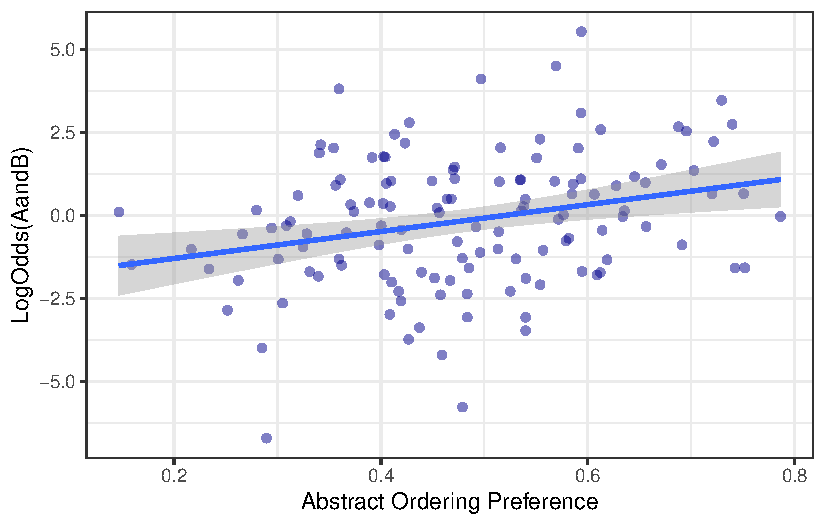
\includegraphics[width=0.8\textwidth,height=\textheight]{nonce_binoms_writeup_files/figure-pdf/fig-exp1m1-1.pdf}

}

\caption{\label{fig-exp1m1}Visualization of the effects of AbsPref on
LogOdds(AandB)}

\end{figure}%

While these results suggest that the large language models' ordering
preferences are sensitive to similar factors as humans, it's unclear
whether this similarity holds on the level of the individual
constraints. Thus, in the second analysis we examine which specific
constraints the model is sensitive to, and to what extent.\footnote{It's
  also helpful to consider how many of our binomials the constraint even
  applied to (i.e., how many binomials were the constraints non-zero).
  For the Culture constraint, 62 of our 131 binomials had a non-zero
  value. For the Power constraint, 54 did, for the Frequency constraint,
  all 131 binomials did, and for the Len constraint, 85 did.} For this
analysis, following Z. Houghton et al. (2024), we also present the
percentage of posterior samples greater than zero. The results of this
analysis can be found below in Table~\ref{tbl-exp1m2}.

\begin{longtable}[]{@{}lllllr@{}}

\caption{\label{tbl-exp1m2}Model results examining the effect of each
individual constraint on LogOdds(AandB).}

\tabularnewline

\toprule\noalign{}
& Estimate & Est.Error & Q2.5 & Q97.5 & \% Samples \textgreater{} 0 \\
\midrule\noalign{}
\endhead
\bottomrule\noalign{}
\endlastfoot
Intercept & -0.132 & 0.163 & -0.451 & 0.185 & 20.750 \\
Culture & 0.414 & 0.254 & -0.078 & 0.916 & 94.945 \\
Power & 0.720 & 0.263 & 0.204 & 1.236 & 99.665 \\
Freq & 0.091 & 0.087 & -0.079 & 0.263 & 85.170 \\
Len & -0.209 & 0.134 & -0.476 & 0.052 & 5.870 \\

\end{longtable}

The model is most sensitive to the Power constraint, however there
appears to be a marginal effect of Culture as well, since nearly 95\% of
the posterior samples are greater than zero despite the credible
interval crossing zero. Surprisingly, there also appears to be a
negative effect of length with a slight preference to place the longer
word first, which is the opposite direction from what we see in humans.
Length is often correlated with frequency, since frequent words tend to
be shorter. As such, we ran a model without frequency to determine
whether the negative effect of length was do to co-linearity with
frequency. However, dropping frequency from the model did not affect the
effect of length. Further, we also ran a model with only length as the
predictor and for that model as well the estimate of length remained
negative.

\subsection{Discussion}\label{discussion}

The present experiment found that OLMo-7B has learned abstract ordering
preferences even for novel binomials that it has never seen before.
Further, these ordering preferences aren't simply based on the
individual word frequencies. Specifically, we find a main-effect of
abstract ordering preferences on the model's binomial ordering
preferences. Additionally, we find a strong preference to place the more
powerful word first, a weak preference to place the more culturally
central word first, and a weak preference to place the longer word
first.

These results together suggest that the model is learning abstract
ordering preferences but these are not identical to humans. For example,
while humans also show a preference for placing the more powerful and
more culturally central words first, humans also prefer to place the
\emph{shorter} word first (Morgan \& Levy, 2015, 2016a). However, we
find the opposite finding: large language models prefer to place the
longer word first. One explanation for this is a difference in terms of
the input between humans and large language models. The length
constraint is determined by the number of syllables. Syllables are
salient cues in the audio that humans receive during learning
{[}\textbf{NEED CITATION{]}}, but it's less clear how salient of a cue
this is for large language models, which receive sub-word tokens (which
vary in their size, from being individual orthographic symbols to being
entire words\footnote{For example, both \emph{ictionary} and
  \emph{region} are individual tokens in OpenAI's models
  (\url{https://gist.github.com/s-macke/ae83f6afb89794350f8d9a1ad8a09193}).}).

\section{Experiment 2}\label{experiment-2}

In Experiment 1 we demonstrated that large language models are not
simply copying their training, but are learning some abstract ordering
preferences from their input. However, OLMo makes public various
checkpoints during the model's training, thus allowing us the
opportunity to examine how these preferences arise as a function of the
training. Thus, in Experiment 2 we examine the evolution of these
learned abstract ordering preferences as the model learns over time.

\subsection{Methods}\label{methods-1}

\subsubsection{Language Model
Predictions}\label{language-model-predictions-1}

Our language model predictions in Experiment 2 were obtained using the
same procedure as in Experiment 1. However, instead of calculating these
metrics only for the main model, we calculated them at various
checkpoints. These checkpoints are listed below, in terms of the steps
as well as the number of billions of tokens the model had been trained
on at that checkpoint:

\begin{itemize}
\item
  Step 0, 0B Tokens
\item
  Step 1000, 2B Tokens
\item
  Step 10000, 41B Tokens
\item
  Step 50000, 209B Tokens
\item
  Step 100000, 419B Tokens
\item
  Step 200000, 838B Tokens
\item
  Step 400000, Tokens 1677B
\end{itemize}

\subsubsection{Analysis}\label{analysis}

We ran the same two analyses as in Experiment 1, however, we ran these
analyses for the each of the checkpoints listed above.

\subsection{Results}\label{results-1}

Our model estimates for the effect of AbsPref on LogOdds(AandB) at each
checkpoint are presented below in Table~\ref{tbl-exp2m1} and visualized
in Figure~\ref{fig-exp2m1}.

\begin{longtable}[]{@{}lllll@{}}

\caption{\label{tbl-exp2m1}Model results examining the effect of AbsPref
on LogOdds(AandB) for each checkpoint.}

\tabularnewline

\toprule\noalign{}
Number of Tokens & Estimate & Est.Error & Q2.5 & Q97.5 \\
\midrule\noalign{}
\endhead
\bottomrule\noalign{}
\endlastfoot
0B & 0.189 & 0.789 & -1.303 & 1.787 \\
2B & 1.210 & 1.346 & -0.944 & 4.404 \\
41B & 0.869 & 1.167 & -1.119 & 3.472 \\
209B & 1.051 & 1.040 & -0.776 & 3.375 \\
419B & 1.700 & 1.216 & -0.355 & 4.326 \\
838B & 1.770 & 1.267 & -0.320 & 4.585 \\
1677B & 3.858 & 1.516 & 0.948 & 6.825 \\

\end{longtable}

The model results are visualized below in Figure~\ref{fig-exp2m1}.

\begin{figure}

\centering{

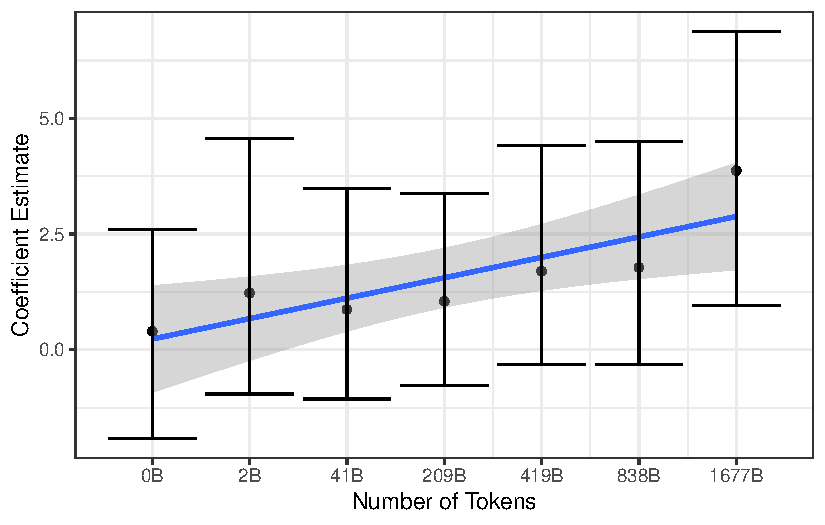
\includegraphics[width=0.7\textwidth,height=\textheight]{nonce_binoms_writeup_files/figure-pdf/fig-exp2m1-1.pdf}

}

\caption{\label{fig-exp2m1}Visualization of the model predictions for
the effect of AbsPref on LogOdds(AandB) for each checkpoint.}

\end{figure}%

Our results demonstrate that it takes quite a large number of tokens for
the model to learn the abstract ordering preferences. As
Figure~\ref{fig-exp2m1} demonstrates, the effect of abstract ordering
preference isn't convincing until the model has experienced 419 billion
tokens. However, it does appear that the model develops a slight
preference quite rapidly. For example, by 2 billion tokens there appears
to be a very slight (though unconvincing) effect of abstract ordering
preferences on the ordering of binomials.

Similar to Experiment 1, in our second analysis we present a breakdown
of the effects of each individual constraint. In this analysis, however,
we demonstrate the effect of each constraint at each checkpoint. The
full table results can be found in the
Section~\ref{sec-individual-constraints-at-each-checkpoint}, but we
present a visualization below in Figure~\ref{fig-exp2m2}.

\begin{figure}

\centering{

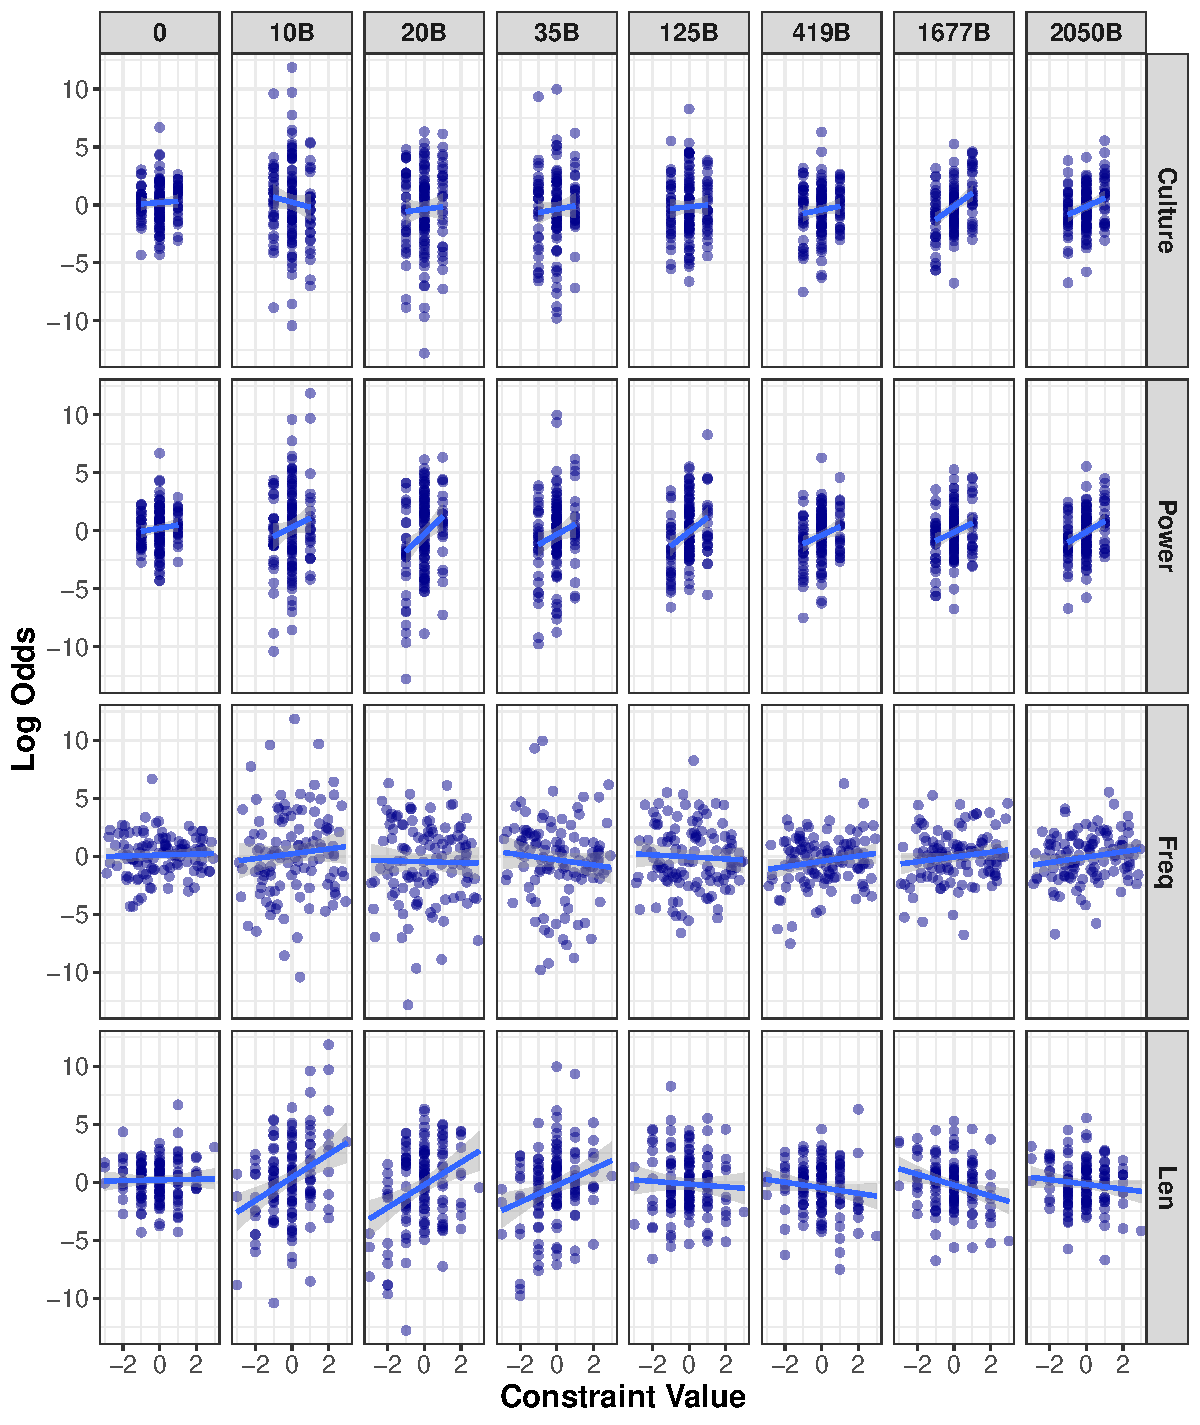
\includegraphics{nonce_binoms_writeup_files/figure-pdf/fig-exp2m2-1.pdf}

}

\caption{\label{fig-exp2m2}Visualization of the effect of each
constraint on the ordering preference at each checkpoint.}

\end{figure}%

Interestingly, it appears that early on the model already shows evidence
of learning human-like preferences. For example, by 10 billion tokens,
the model has learned to place more powerful words first and shorter
words first. However, the model seems slower to learn to place more
culturally central words first. Further, as it receives more training
the effect of length undergoes a reversal in direction.

\subsection{Discussion}\label{discussion-1}

Our results demonstrate that OLMo learns human-like ordering preferences
early on for most of the constraints, but takes longer to learn
human-like ordering preferences for the culture constraint. Further, the
model is human-like in its predictions for length early on, but as it
receives more training data it learns the opposite length prediction. It
is unclear what exactly is causing this reversal, but as we suggested
earlier it may be a function of the tokenization differences between
human input and large language models' input. We look forward to
examining this question in more depth in future studies.

Our results can also be interpreted as predictions for human data. For
example, it takes the model longer to learn the Culture constraint than
the other constraints. Is the same true for humans?

Finally, previous results suggest that for non-novel binomials that OLMo
has experienced before, it relies almost exclusively on its experience
with it in its training data (i.e., its ordering preference is primarily
driven by the proportion of occurrences in alphabetical to
nonalphabetical ordering) and does not use abstract ordering preferences
at all (Z. N. Houghton et al., 2025). Our results thus suggest that
while large language models are able to learn abstract ordering
preferences, in cases where they've seen the binomial they are able to
rely on their experience more than a human can.

\section{Conclusion}\label{conclusion}

In the present study, we examined the ordering preferences in OLMo 7B's
main model as well as the model at various stages in learning. We found
that the main model shows human-like ordering preferences, with the
exception of a preference for longer words before shorter words.
Further, we show that while the effect of abstract ordering preference
on a whole takes a great deal of time (over 400 billion tokens to be
convincing), the model seems to pick up on individual constraints quite
early on, and initially even learns the correct direction of the length
constraint.

Our results suggest that large language models are not simply copying
their input, but are learning interesting, human-like phenomena from
their training. However, they are not learning identically to humans, as
demonstrated by the opposite direction of the length preference. This is
not surprising given the differences in tokenization methods. Further,
while humans rely on abstract preferences even for binomials that they
have encountered before, large language models only rely on abstract
ordering preferences for items that they have not encountered at all.

\section{Limitations}\label{limitations}

The main limitation is the number of models tested. We only tested one
model in this study, so it's possible that other large language models
may demonstrate different ordering preferences. However, we believe that
the advantages of demonstrating an in-depth analysis of a single model
outweigh a more broad analysis of several models, especially given the
lack of easily available open access training data, which is crucial to
guaranteeing that the model has not encountered our items before.

Additionally, we only test one construction in this paper (binomials).
While it is possible that abstract ordering preferences for binomials
are different than other constructions, binomials are well understood in
the human linguistics literature thus making them a good test case for
our analyses.

\clearpage

\section*{References}\label{references}
\addcontentsline{toc}{section}{References}

\bibliographystyle{acl_natbib.bst}

\phantomsection\label{refs}
\begin{CSLReferences}{1}{0}
\bibitem[\citeproctext]{ref-ambridge2020}
Ambridge, B. (2020). Against stored abstractions: A radical exemplar
model of language acquisition. \emph{First Language}, \emph{40}(5-6),
509--559. \url{https://doi.org/10.1177/0142723719869731}

\bibitem[\citeproctext]{ref-benderDangersStochasticParrots2021}
Bender, E. M., Gebru, T., McMillan-Major, A., \& Shmitchell, S. (2021).
\emph{FAccT '21: 2021 ACM Conference on Fairness, Accountability, and
Transparency}. 610--623. \url{https://doi.org/10.1145/3442188.3445922}

\bibitem[\citeproctext]{ref-bender2020climbing}
Bender, E. M., \& Koller, A. (2020). Climbing towards NLU: On meaning,
form, and understanding in the age of data. \emph{Proceedings of the
58th Annual Meeting of the Association for Computational Linguistics},
5185--5198.

\bibitem[\citeproctext]{ref-benorChickenEggProbabilistic2006}
Benor, S. B., \& Levy, R. (2006). The chicken or the egg? A
probabilistic analysis of english binomials. \emph{Language},
\emph{82}(2), 233--278. \url{https://doi.org/10.1353/lan.2006.0077}

\bibitem[\citeproctext]{ref-berko}
Berko, J. (1958). The Child's Learning of English Morphology.
\emph{{\emph{WORD}}}, \emph{14}(2-3), 150--177.
\url{https://doi.org/10.1080/00437956.1958.11659661}

\bibitem[\citeproctext]{ref-brms}
Bürkner, P.-C. (2017). Brms: An r package for bayesian multilevel models
using stan. \emph{Journal of Statistical Software}, \emph{80}, 128.
\url{https://www.jstatsoft.org/article/view/v080i01}

\bibitem[\citeproctext]{ref-cooper1975world}
Cooper, W. E., \& Ross, J. R. (1975). World order. \emph{Papers from the
Parasession on Functionalism}, \emph{11}, 63--111.

\bibitem[\citeproctext]{ref-groeneveldOLMoAcceleratingScience2024}
Groeneveld, D., Beltagy, I., Walsh, P., Bhagia, A., Kinney, R., Tafjord,
O., Jha, A. H., Ivison, H., Magnusson, I., Wang, Y., et al. (2024).
Olmo: Accelerating the science of language models. \emph{arXiv Preprint
arXiv:2402.00838}.

\bibitem[\citeproctext]{ref-haley2020bert}
Haley, C. (2020). This is a BERT. Now there are several of them. Can
they generalize to novel words? \emph{Proceedings of the Third
BlackboxNLP Workshop on Analyzing and Interpreting Neural Networks for
NLP}, 333--341.

\bibitem[\citeproctext]{ref-HoughtonMorgan2025}
Houghton, Z. N., Sagae, K., \& Morgan, E. (2025). \emph{The role of
abstract representations and observed preferences in the ordering of
binomials in large language models}. University of California, Davis.

\bibitem[\citeproctext]{ref-houghtonTaskdependentConsequencesDisfluency2024}
Houghton, Z., Kato, M., Baese-Berk, M., \& Vaughn, C. (2024).
Task-dependent consequences of disfluency in perception of native and
non-native speech. \emph{Applied Psycholinguistics}, 1--17.
\url{https://doi.org/10.1017/S0142716423000486}

\bibitem[\citeproctext]{ref-lasri2022subject}
Lasri, K., Seminck, O., Lenci, A., \& Poibeau, T. (2022). Subject verb
agreement error patterns in meaningless sentences: Humans vs. BERT.
\emph{arXiv Preprint arXiv:2209.10538}.

\bibitem[\citeproctext]{ref-lebrun2022evaluating}
LeBrun, B., Sordoni, A., \& O'Donnell, T. J. (2022). Evaluating
distributional distortion in neural language modeling. \emph{arXiv
Preprint arXiv:2203.12788}.

\bibitem[\citeproctext]{ref-levy2012}
Levy, R., Fedorenko, E., Breen, M., \& Gibson, E. (2012). The processing
of extraposed structures in english. \emph{Cognition}, \emph{122}(1),
12--36. \url{https://doi.org/10.1016/j.cognition.2011.07.012}

\bibitem[\citeproctext]{ref-liAreNeuralNetworks2021}
Li, B., \& Wisniewski, G. (2021). \emph{Are neural networks extracting
linguistic properties or memorizing training data? An observation with a
multilingual probe for predicting tense}.
\url{https://shs.hal.science/halshs-03197072/}

\bibitem[\citeproctext]{ref-liAssessingCapacityTransformer2023}
Li, B., Wisniewski, G., \& Crabbé, B. (2023). Assessing the capacity of
transformer to abstract syntactic representations: A contrastive
analysis based on long-distance agreement. \emph{Transactions of the
Association for Computational Linguistics}, \emph{11}, 18--33.
\url{https://doi.org/10.1162/tacl_a_00531}

\bibitem[\citeproctext]{ref-mccoyUniversalLinguisticInductive2020}
McCoy, R. T., Grant, E., Smolensky, P., Griffiths, T. L., \& Linzen, T.
(n.d.). \emph{Universal linguistic inductive biases via meta-learning}.
\url{https://doi.org/10.48550/arXiv.2006.16324}

\bibitem[\citeproctext]{ref-mccoy2023much}
McCoy, R. T., Smolensky, P., Linzen, T., Gao, J., \& Celikyilmaz, A.
(2023). How much do language models copy from their training data?
Evaluating linguistic novelty in text generation using raven.
\emph{Transactions of the Association for Computational Linguistics},
\emph{11}, 652--670.

\bibitem[\citeproctext]{ref-morganModelingIdiosyncraticPreferences2015}
Morgan, E., \& Levy, R. (2015). \emph{Modeling idiosyncratic preferences
: How generative knowledge and expression frequency jointly determine
language structure}. 1649--1654.

\bibitem[\citeproctext]{ref-morganAbstractKnowledgeDirect2016}
Morgan, E., \& Levy, R. (2016a). Abstract knowledge versus direct
experience in processing of binomial expressions. \emph{Cognition},
\emph{157}, 384--402.
\url{https://doi.org/10.1016/j.cognition.2016.09.011}

\bibitem[\citeproctext]{ref-morganFrequencydependentRegularizationIterated2016a}
Morgan, E., \& Levy, R. (2016b). Frequency-dependent regularization in
iterated learning. \emph{The Evolution of Language: Proceedings of the
11th International Conference}.

\bibitem[\citeproctext]{ref-morganProductiveKnowledgeItemspecific2024}
Morgan, E., \& Levy, R. (2024). Productive knowledge and item-specific
knowledge trade off as a function of frequency in multiword expression
processing. \emph{Language}, \emph{100}(4), e195--e224.
\url{https://muse.jhu.edu/pub/24/article/947046}

\bibitem[\citeproctext]{ref-piantadosiChapterModernLanguage}
Piantadosi, S. T. (2023). Modern language models refute chomsky's
approach to language. \emph{From Fieldwork to Linguistic Theory: A
Tribute to Dan Everett}, 353--414.

\bibitem[\citeproctext]{ref-piantadosiMeaningReferenceLarge2022}
Piantadosi, S. T., \& Hill, F. (2022). Meaning without reference in
large language models. \emph{arXiv Preprint arXiv:2208.02957}.

\bibitem[\citeproctext]{ref-soldainiDolmaOpenCorpus2024}
Soldaini, L., Kinney, R., Bhagia, A., Schwenk, D., Atkinson, D., Authur,
R., Bogin, B., Chandu, K., Dumas, J., Elazar, Y., et al. (2024). Dolma:
An open corpus of three trillion tokens for language model pretraining
research. \emph{arXiv Preprint arXiv:2402.00159}.

\bibitem[\citeproctext]{ref-tartaglini2023deep}
Tartaglini, A. R., Feucht, S., Lepori, M. A., Vong, W. K., Lovering, C.,
Lake, B. M., \& Pavlick, E. (2023). Deep neural networks can learn
generalizable same-different visual relations. \emph{arXiv Preprint
arXiv:2310.09612}.

\bibitem[\citeproctext]{ref-nyt_v_openai}
\emph{{The New York Times Company v. Microsoft Corporation, OpenAI,
Inc., OpenAI LP, OpenAI GP, LLC, OpenAI, LLC, OpenAI OpCo LLC, OpenAI
Global LLC, OAI Corporation, LLC, and OpenAI Holdings, LLC}}. (2024).
Civil Action No. 1:23-cv-11195-SHS, United States District Court,
Southern District of New York, May 31, 2024.

\bibitem[\citeproctext]{ref-yu2007rapid}
Yu, C., \& Smith, L. B. (2007). Rapid word learning under uncertainty
via cross-situational statistics. \emph{Psychological Science},
\emph{18}(5), 414--420.

\bibitem[\citeproctext]{ref-zhengTakeStepBack2024}
Zheng, H. S., Mishra, S., Chen, X., Cheng, H.-T., Chi, E. H., Le, Q. V.,
\& Zhou, D. (n.d.). \emph{Take a step back: Evoking reasoning via
abstraction in large language models}.
\url{https://doi.org/10.48550/arXiv.2310.06117}

\end{CSLReferences}

\newpage

\section*{Appendices}\label{appendices}
\addcontentsline{toc}{section}{Appendices}

\appendix

\renewcommand{\thesection}{\Alph{section}}

\setcounter{section}{0}

\counterwithin{figure}{section}

\counterwithin{table}{section}

\section{Full List of Stimuli}\label{sec-full-list-of-stimuli}

Below is a table of our list of binomials as well as the individual
constraint values for each.

\begin{longtable}[]{@{}
  >{\raggedright\arraybackslash}p{(\columnwidth - 24\tabcolsep) * \real{0.1415}}
  >{\raggedright\arraybackslash}p{(\columnwidth - 24\tabcolsep) * \real{0.1226}}
  >{\raggedleft\arraybackslash}p{(\columnwidth - 24\tabcolsep) * \real{0.0472}}
  >{\raggedleft\arraybackslash}p{(\columnwidth - 24\tabcolsep) * \real{0.0755}}
  >{\raggedleft\arraybackslash}p{(\columnwidth - 24\tabcolsep) * \real{0.0755}}
  >{\raggedleft\arraybackslash}p{(\columnwidth - 24\tabcolsep) * \real{0.0566}}
  >{\raggedleft\arraybackslash}p{(\columnwidth - 24\tabcolsep) * \real{0.0755}}
  >{\raggedleft\arraybackslash}p{(\columnwidth - 24\tabcolsep) * \real{0.0472}}
  >{\raggedleft\arraybackslash}p{(\columnwidth - 24\tabcolsep) * \real{0.0660}}
  >{\raggedleft\arraybackslash}p{(\columnwidth - 24\tabcolsep) * \real{0.0377}}
  >{\raggedleft\arraybackslash}p{(\columnwidth - 24\tabcolsep) * \real{0.0566}}
  >{\raggedleft\arraybackslash}p{(\columnwidth - 24\tabcolsep) * \real{0.1226}}
  >{\raggedleft\arraybackslash}p{(\columnwidth - 24\tabcolsep) * \real{0.0755}}@{}}

\caption{\label{tbl-stimuli}Full list of binomials as well as their
constraints.}

\tabularnewline

\toprule\noalign{}
\begin{minipage}[b]{\linewidth}\raggedright
Word1
\end{minipage} & \begin{minipage}[b]{\linewidth}\raggedright
Word2
\end{minipage} & \begin{minipage}[b]{\linewidth}\raggedleft
Form
\end{minipage} & \begin{minipage}[b]{\linewidth}\raggedleft
Percept
\end{minipage} & \begin{minipage}[b]{\linewidth}\raggedleft
Culture
\end{minipage} & \begin{minipage}[b]{\linewidth}\raggedleft
Power
\end{minipage} & \begin{minipage}[b]{\linewidth}\raggedleft
Intense
\end{minipage} & \begin{minipage}[b]{\linewidth}\raggedleft
Icon
\end{minipage} & \begin{minipage}[b]{\linewidth}\raggedleft
Freq
\end{minipage} & \begin{minipage}[b]{\linewidth}\raggedleft
Len
\end{minipage} & \begin{minipage}[b]{\linewidth}\raggedleft
Lapse
\end{minipage} & \begin{minipage}[b]{\linewidth}\raggedleft
Final Stress
\end{minipage} & \begin{minipage}[b]{\linewidth}\raggedleft
AbsPref
\end{minipage} \\
\midrule\noalign{}
\endhead
\bottomrule\noalign{}
\endlastfoot
kiwis & wolverines & 0 & 0 & 0 & -1 & -1 & 0 & -0.291 & 1 & -1 & -1 &
0.427 \\
kiwis & narwhals & 0 & 1 & 0 & -1 & -1 & 0 & 2.715 & 0 & -1 & -1 &
0.515 \\
kiwis & ocelots & 0 & 0 & 0 & -1 & 0 & 0 & 2.737 & 0 & -1 & -1 &
0.458 \\
ibex & kiwis & 0 & 0 & 0 & 1 & 0 & 0 & -1.171 & 0 & 1 & 0 & 0.497 \\
harpies & kiwis & 0 & -1 & 0 & 1 & 1 & 0 & -1.948 & 0 & 0 & 0 & 0.471 \\
axolotls & wolverines & 0 & -1 & 0 & -1 & 0 & 0 & -2.689 & -1 & -1 & -1
& 0.262 \\
axolotls & ibex & 0 & -1 & 0 & -1 & 0 & 0 & -1.228 & -2 & -1 & 0 &
0.331 \\
axolotls & harpies & 0 & 1 & 0 & -1 & -1 & 0 & -0.450 & -2 & 0 & 0 &
0.413 \\
axolotls & keas & 0 & 0 & 1 & -1 & 0 & 0 & 1.052 & -3 & -1 & 1 &
0.591 \\
axolotls & bonobos & 0 & -1 & 0 & -1 & 0 & 0 & -0.895 & -1 & 0 & 0 &
0.328 \\
axolotls & wombats & 0 & -1 & 0 & -1 & 0 & 0 & -0.655 & -2 & -1 & -1 &
0.266 \\
axolotls & lions & 0 & -1 & -1 & -1 & -1 & 0 & -5.114 & -2 & 0 & 0 &
0.159 \\
ocelots & platypuses & 0 & 1 & -1 & 1 & 0 & 0 & 0.665 & 1 & 3 & 1 &
0.525 \\
ibex & platypuses & 0 & 1 & 0 & 1 & 0 & 0 & 2.232 & 2 & 3 & 1 & 0.691 \\
harpies & platypuses & 0 & 0 & 0 & 1 & 1 & 0 & 1.454 & 2 & 2 & 0 &
0.585 \\
keas & platypuses & 0 & 0 & -1 & 0 & 0 & 0 & -0.048 & 3 & 3 & 1 &
0.459 \\
bonobos & platypuses & 0 & 1 & 0 & 1 & 0 & 0 & 1.898 & 1 & 2 & 0 &
0.612 \\
harpies & wolverines & 0 & -1 & 0 & 0 & 0 & 0 & -2.239 & 1 & -1 & 1 &
0.571 \\
keas & wolverines & 0 & -1 & -1 & -1 & 0 & 0 & -3.741 & 2 & 0 & 0 &
0.285 \\
bonobos & wolverines & 0 & 0 & 0 & 0 & 0 & 0 & -1.795 & 0 & -1 & -1 &
0.426 \\
capybaras & ibex & 0 & 0 & 0 & 0 & 0 & 0 & -1.659 & -2 & -1 & -1 &
0.356 \\
capybaras & harpies & 0 & 1 & 0 & -1 & -1 & 0 & -0.882 & -2 & 0 & 0 &
0.404 \\
capybaras & keas & 0 & 1 & 1 & 1 & 0 & 0 & 0.621 & -3 & -1 & -1 &
0.593 \\
ibex & narwhals & 0 & 1 & 0 & -1 & 0 & 0 & 1.544 & 0 & 0 & 0 & 0.536 \\
harpies & narwhals & 0 & -1 & 0 & 0 & 1 & 0 & 0.767 & 0 & -1 & -1 &
0.423 \\
keas & narwhals & 0 & 0 & -1 & -1 & 0 & 0 & -0.736 & 1 & 0 & 0 &
0.362 \\
ibex & ocelots & 0 & 0 & 0 & 0 & 0 & 0 & 1.566 & 1 & 0 & 0 & 0.576 \\
keas & ocelots & 0 & -1 & -1 & -1 & 0 & 0 & -0.714 & 2 & 0 & 0 &
0.340 \\
bonobos & ocelots & 0 & 0 & 1 & 0 & 0 & 0 & 1.233 & 0 & -1 & -1 &
0.594 \\
harpies & ibex & 0 & -1 & 0 & 0 & 1 & 0 & -0.777 & 0 & -1 & -1 &
0.391 \\
ibex & keas & 0 & 1 & 1 & 1 & 0 & 0 & 2.280 & -1 & 0 & 0 & 0.729 \\
bonobos & ibex & 0 & 0 & 0 & 0 & 0 & 0 & -0.333 & -1 & -1 & -1 &
0.419 \\
ibex & koalas & 0 & 0 & -1 & 0 & 0 & 0 & -0.433 & 1 & 1 & 1 & 0.471 \\
ibex & sloths & 0 & 0 & -1 & 1 & 0 & 0 & -0.035 & -1 & 0 & 0 & 0.427 \\
aardvarks & ibex & 0 & 0 & 1 & 0 & 0 & 0 & -1.945 & 0 & 0 & 0 & 0.568 \\
harpies & keas & 0 & -1 & 1 & 1 & 1 & 0 & 1.503 & -1 & -1 & -1 &
0.569 \\
bonobos & harpies & 0 & 1 & 0 & -1 & -1 & 0 & 0.444 & -1 & 0 & 0 &
0.470 \\
harpies & koalas & 0 & -1 & -1 & 0 & 1 & 0 & -1.210 & 1 & 0 & 0 &
0.359 \\
harpies & wombats & 0 & -1 & 0 & 1 & 1 & 0 & -0.204 & 0 & -1 & -1 &
0.467 \\
aardvarks & harpies & 0 & 1 & 0 & 0 & -1 & 0 & -1.167 & 0 & 1 & 1 &
0.579 \\
bonobos & keas & 0 & 1 & 1 & 1 & 0 & 0 & 1.947 & -2 & -1 & -1 & 0.656 \\
keas & koalas & 0 & -1 & -1 & -1 & 0 & 0 & -2.712 & 2 & 1 & 1 & 0.339 \\
keas & sloths & 0 & -1 & -1 & 0 & 0 & 0 & -2.315 & 0 & 0 & 0 & 0.301 \\
keas & wombats & 0 & -1 & -1 & -1 & 0 & 0 & -1.707 & 1 & 0 & 0 &
0.289 \\
keas & lions & 0 & -1 & -1 & -1 & -1 & 0 & -6.166 & 0 & 1 & 1 & 0.217 \\
aardvarks & keas & 0 & 1 & 1 & 1 & 0 & 0 & 0.335 & -1 & 0 & 0 & 0.695 \\
bonobos & wombats & 0 & 0 & 0 & 1 & 0 & 0 & 0.240 & -1 & -1 & -1 &
0.496 \\
aardvarks & bonobos & 0 & 0 & 0 & 0 & 0 & 0 & -1.611 & 1 & 1 & 1 &
0.551 \\
ocarinas & vibraphones & 0 & 0 & 1 & 0 & 0 & 0 & 0.461 & -1 & -1 & -1 &
0.540 \\
cymbals & ocarinas & 0 & 0 & 1 & 1 & 0 & 0 & 3.485 & 2 & 0 & 0 &
0.786 \\
clarinets & ocarinas & 0 & 0 & 1 & 1 & 0 & 0 & 2.245 & 0 & 1 & 1 &
0.742 \\
cellos & ocarinas & 0 & 0 & 1 & 0 & 0 & 0 & 2.344 & 2 & 0 & 0 & 0.720 \\
didgeridoos & vibraphones & 0 & 0 & 0 & 0 & 0 & 0 & 0.533 & -1 & 0 & 0 &
0.479 \\
lutes & marimbas & 0 & 0 & 0 & 0 & 0 & 0 & 1.225 & 2 & 1 & 1 & 0.645 \\
kalimbas & lutes & 0 & 0 & 0 & 0 & 0 & 0 & -2.407 & -2 & -1 & -1 &
0.342 \\
clarinets & kalimbas & 0 & 0 & 1 & 1 & 0 & 0 & 2.827 & 0 & 1 & 1 &
0.752 \\
kalimbas & trumpets & 0 & 0 & -1 & -1 & 0 & 0 & -4.437 & -1 & 0 & 0 &
0.234 \\
cellos & kalimbas & 0 & 0 & 1 & 1 & 0 & 0 & 2.926 & 1 & 0 & 0 & 0.751 \\
kalimbas & saxophones & 0 & 0 & -1 & -1 & 0 & 0 & -3.124 & 0 & -1 & -1 &
0.252 \\
lutes & saxophones & 0 & 0 & -1 & -1 & 0 & 0 & -0.717 & 2 & 0 & 0 &
0.398 \\
casserole & eagle & 0 & -1 & 0 & 0 & -1 & 0 & -1.526 & -1 & 1 & 1 &
0.410 \\
kite & linguist & 0 & -1 & 1 & 0 & 0 & 0 & 1.602 & 1 & 1 & 1 & 0.656 \\
algorithm & perfume & 0 & -1 & -1 & 0 & 0 & 0 & 1.992 & -2 & -1 & -1 &
0.280 \\
forest & screwdriver & 0 & 0 & 0 & 0 & 0 & 0 & 3.294 & 1 & 0 & 0 &
0.612 \\
slipper & volcano & 0 & 0 & 1 & -1 & -1 & 0 & -1.806 & 1 & 0 & 0 &
0.540 \\
harmonica & microscope & 0 & 0 & 0 & 0 & 0 & 0 & -1.745 & -1 & -2 & -1 &
0.437 \\
cookbook & zenith & 0 & 1 & 1 & 0 & 0 & 0 & 1.136 & 0 & 1 & 1 & 0.722 \\
hammock & hydrogen & 0 & 1 & -1 & 0 & 0 & 0 & -2.060 & 1 & 1 & 0 &
0.410 \\
neuron & toaster & 0 & -1 & -1 & 0 & 0 & 0 & 0.383 & 0 & 1 & 0 &
0.309 \\
marshmallow & telescope & 0 & 0 & 0 & 0 & 0 & 0 & -1.166 & 0 & -1 & -1 &
0.439 \\
casserole & optics & 0 & 1 & 0 & 0 & 0 & 0 & -0.665 & -1 & 1 & 1 &
0.557 \\
encyclopedia & comet & 0 & 1 & 0 & -1 & 0 & 0 & 0.947 & -4 & -1 & 0 &
0.420 \\
nimbus & waffle & 0 & -1 & -1 & 0 & 0 & 0 & -1.680 & 0 & 0 & 0 &
0.312 \\
photon & pumpkin & 0 & -1 & -1 & 0 & 0 & 0 & -0.793 & 0 & 1 & 1 &
0.367 \\
lantern & syntax & 0 & 1 & 1 & 0 & 0 & 0 & -0.941 & 0 & -1 & -1 &
0.609 \\
echo & vineyard & 0 & -1 & 0 & 0 & 0 & 0 & 1.884 & 0 & 0 & 0 & 0.484 \\
nebula & snowman & 0 & -1 & -1 & 0 & 0 & 0 & 0.182 & -1 & -2 & -1 &
0.320 \\
botany & teapot & 0 & -1 & -1 & 0 & 0 & 0 & 0.438 & -1 & -2 & -1 &
0.325 \\
chisel & kaleidoscope & 0 & 0 & 0 & 1 & 0 & 0 & 0.139 & 2 & -1 & -1 &
0.606 \\
lava & teacup & 0 & -1 & -1 & 1 & 0 & 0 & 1.969 & 0 & -1 & -1 & 0.405 \\
entropy & orchard & 0 & -1 & -1 & 0 & 0 & 0 & 0.370 & -1 & -1 & 0 &
0.361 \\
axolotl & vineyard & 0 & 1 & 0 & 0 & 0 & 0 & -3.510 & -2 & 0 & 0 &
0.417 \\
clockwork & meadow & 0 & -1 & 0 & 0 & 0 & 0 & -0.987 & 0 & 1 & 1 &
0.464 \\
algebra & telescope & 0 & -1 & 0 & 0 & 0 & 0 & 8.751 & 0 & -2 & -1 &
0.634 \\
arcade & topaz & 0 & 0 & 0 & 0 & 0 & 0 & 2.276 & 0 & 0 & 0 & 0.554 \\
asteroid & compass & 0 & -1 & 0 & 1 & 0 & 0 & -0.862 & -1 & 0 & 0 &
0.452 \\
bicycle & nebula & 0 & 1 & 1 & 0 & 0 & 0 & 1.991 & 0 & 0 & 0 & 0.703 \\
bungalow & entropy & 0 & 1 & 0 & 0 & 0 & 0 & -1.198 & 0 & 2 & 1 &
0.535 \\
carnation & gnome & 0 & 0 & 0 & 0 & 0 & 0 & -1.769 & -2 & -1 & -1 &
0.354 \\
cinnamon & harmonica & 0 & 0 & 1 & 0 & 0 & 0 & 2.300 & 1 & 0 & 0 &
0.688 \\
coral & syntax & 0 & 1 & 1 & 0 & 0 & 0 & -0.020 & 0 & -1 & -1 & 0.627 \\
dandelion & pendulum & 0 & 0 & 0 & 0 & 0 & 0 & -0.533 & -1 & 1 & 0 &
0.409 \\
delirium & telescope & 0 & -1 & -1 & 0 & 1 & 0 & -1.442 & -1 & -2 & -1 &
0.294 \\
anchors & sandstorms & 0 & 1 & 0 & 0 & -1 & 0 & 3.416 & 0 & -1 & -1 &
0.593 \\
scissors & volcanoes & 0 & 0 & 1 & -1 & 0 & 0 & 0.577 & 1 & 0 & 0 &
0.594 \\
equations & lanterns & 0 & -1 & 0 & 0 & 0 & 0 & 2.297 & -1 & 0 & 0 &
0.454 \\
satellites & tulips & 0 & -1 & 0 & 0 & 0 & 0 & 1.493 & -1 & 1 & 1 &
0.479 \\
compasses & hedgehogs & 0 & -1 & 0 & 0 & 0 & 0 & -0.612 & -1 & -2 & -1 &
0.400 \\
comets & neckties & 0 & -1 & 0 & 1 & 0 & 0 & 2.294 & 0 & -1 & -1 &
0.516 \\
castles & headphones & 0 & 0 & -1 & 1 & 0 & 0 & -1.098 & 0 & -1 & -1 &
0.402 \\
paperclips & pyramids & 0 & 0 & 1 & -1 & 0 & 0 & -2.884 & 0 & 0 & 0 &
0.483 \\
constellations & kettles & 0 & -1 & 0 & 0 & 0 & 0 & 0.938 & -2 & 0 & 0 &
0.389 \\
kaleidoscopes & whales & 0 & -1 & -1 & -1 & 0 & 0 & -4.654 & -3 & 0 & 0
& 0.147 \\
meadows & pianos & 0 & -1 & -1 & 0 & 0 & 0 & 1.147 & 1 & 0 & 0 &
0.403 \\
magnets & zebras & 0 & -1 & 1 & 0 & 0 & 0 & 1.821 & 0 & 0 & 0 & 0.586 \\
parrots & submarines & 0 & 1 & 0 & -1 & 0 & 0 & -0.346 & 1 & -1 & -1 &
0.492 \\
crayons & jungles & 0 & 1 & 1 & 0 & 0 & 0 & 0.286 & 0 & 0 & 0 & 0.671 \\
harbor & teapot & 0 & -1 & 0 & 0 & 0 & 0 & 2.561 & 0 & -1 & -1 &
0.457 \\
notebook & quicksand & 0 & 0 & 1 & -1 & 0 & 0 & 3.309 & 0 & 0 & 0 &
0.614 \\
glacier & lantern & 0 & -1 & 0 & 0 & 0 & 0 & 0.285 & 0 & 0 & 0 &
0.450 \\
microscope & puddle & 0 & 0 & 0 & 0 & 0 & 0 & 1.361 & -1 & 1 & 1 &
0.538 \\
compass & swan & 0 & -1 & 0 & 0 & 0 & 0 & 0.199 & -1 & -1 & -1 &
0.371 \\
bonsai & cathedral & 0 & 1 & 0 & -1 & 0 & 0 & -2.004 & 1 & 1 & 1 &
0.540 \\
honeycomb & violin & 0 & 0 & -1 & 0 & 0 & 0 & -1.398 & 0 & 0 & 0 &
0.374 \\
sailboat & stadium & 0 & 0 & 0 & 0 & 0 & 0 & -3.213 & 1 & 2 & 1 &
0.468 \\
acorns & skyscrapers & 0 & 1 & 0 & 0 & 0 & 0 & -0.399 & 1 & 1 & 1 &
0.635 \\
bell & trellis & 0 & 0 & 1 & 0 & 0 & 0 & 3.327 & 1 & 1 & 1 & 0.740 \\
inkwell & kite & 0 & 0 & -1 & 0 & 0 & 0 & -3.215 & -1 & 0 & 0 & 0.305 \\
foxglove & trombone & 0 & 0 & -1 & 0 & 0 & 0 & -1.888 & 0 & 1 & 1 &
0.403 \\
carousel & quill & 0 & 0 & 1 & 0 & 0 & 0 & 0.942 & -2 & 0 & 0 & 0.554 \\
lighthouse & onion & 0 & -1 & -1 & 0 & 0 & 0 & -1.153 & 0 & 1 & 1 &
0.359 \\
cactus & chessboard & 0 & 0 & 0 & 0 & 1 & 0 & 2.084 & 0 & -1 & -1 &
0.513 \\
gallery & raindrop & 0 & 0 & 0 & 0 & 0 & 0 & 5.058 & -1 & -2 & -1 &
0.582 \\
cricket & plow & 0 & 1 & 0 & -1 & 0 & 0 & 2.370 & -1 & -1 & -1 &
0.474 \\
gingerbread & fresco & 0 & 0 & 1 & 0 & 0 & 0 & 0.345 & -1 & 1 & 1 &
0.619 \\
cello & sunflower & 0 & 0 & 0 & 0 & 0 & 0 & -0.417 & 1 & 0 & 0 &
0.535 \\
archway & quilt & 0 & 0 & 0 & 0 & 0 & 0 & -2.775 & -1 & 0 & 0 & 0.409 \\
compass & haystack & 0 & 0 & 0 & 0 & 0 & 0 & 2.338 & 0 & -1 & -1 &
0.514 \\
beacon & millipede & 0 & -1 & 0 & 0 & 1 & 0 & 4.030 & 1 & -1 & -1 &
0.531 \\
parchment & windmill & 0 & 0 & 0 & 0 & 0 & 0 & 0.990 & 0 & -1 & -1 &
0.485 \\
candlestick & meadow & 0 & 1 & 0 & 0 & 0 & 0 & -1.463 & -1 & 1 & 1 &
0.540 \\

\end{longtable}

\clearpage

\section{Individual Constraints at Each
Checkpoint}\label{sec-individual-constraints-at-each-checkpoint}

Below is a table of the fixed-effects for each individual constraint at
each checkpoint.

\begin{longtable}[]{@{}llllll@{}}

\caption{\label{tbl-exp2m2}Model results examining the effect of each
individual constraint on LogOdds(AandB).}

\tabularnewline

\toprule\noalign{}
Parameter & num\_tokens & Estimate & Est.Error & Q2.5 & Q97.5 \\
\midrule\noalign{}
\endhead
\bottomrule\noalign{}
\endlastfoot
Intercept & 0B & 0.223 & 0.159 & -0.087 & 0.539 \\
Culture & 0B & 0.149 & 0.244 & -0.327 & 0.623 \\
Power & 0B & 0.286 & 0.249 & -0.207 & 0.777 \\
Freq & 0B & -0.070 & 0.082 & -0.232 & 0.091 \\
Len & 0B & 0.030 & 0.127 & -0.220 & 0.278 \\
Intercept & 2B & -0.027 & 0.256 & -0.529 & 0.478 \\
Culture & 2B & -0.399 & 0.390 & -1.161 & 0.361 \\
Power & 2B & 0.531 & 0.404 & -0.250 & 1.334 \\
Freq & 2B & 0.258 & 0.135 & -0.008 & 0.524 \\
Len & 2B & 0.492 & 0.212 & 0.076 & 0.909 \\
Intercept & 41B & 0.179 & 0.229 & -0.268 & 0.628 \\
Culture & 41B & -0.377 & 0.347 & -1.065 & 0.305 \\
Power & 41B & 1.290 & 0.373 & 0.568 & 2.037 \\
Freq & 41B & -0.035 & 0.121 & -0.274 & 0.202 \\
Len & 41B & 0.807 & 0.188 & 0.438 & 1.179 \\
Intercept & 209B & 0.176 & 0.182 & -0.186 & 0.537 \\
Culture & 209B & 0.290 & 0.283 & -0.268 & 0.847 \\
Power & 209B & 0.760 & 0.289 & 0.194 & 1.327 \\
Freq & 209B & -0.056 & 0.096 & -0.244 & 0.132 \\
Len & 209B & -0.063 & 0.150 & -0.358 & 0.234 \\
Intercept & 419B & -0.458 & 0.183 & -0.816 & -0.099 \\
Culture & 419B & -0.125 & 0.282 & -0.679 & 0.437 \\
Power & 419B & 0.508 & 0.289 & -0.056 & 1.073 \\
Freq & 419B & 0.240 & 0.096 & 0.053 & 0.431 \\
Len & 419B & -0.298 & 0.150 & -0.591 & -0.005 \\
Intercept & 838B & -0.022 & 0.184 & -0.381 & 0.335 \\
Culture & 838B & -0.111 & 0.284 & -0.661 & 0.446 \\
Power & 838B & 0.865 & 0.297 & 0.283 & 1.456 \\
Freq & 838B & 0.127 & 0.099 & -0.068 & 0.319 \\
Len & 838B & 0.247 & 0.154 & -0.055 & 0.552 \\
Intercept & 1677B & -0.181 & 0.176 & -0.527 & 0.159 \\
Culture & 1677B & 0.861 & 0.273 & 0.326 & 1.394 \\
Power & 1677B & 0.562 & 0.275 & 0.031 & 1.108 \\
Freq & 1677B & 0.052 & 0.091 & -0.125 & 0.230 \\
Len & 1677B & -0.431 & 0.142 & -0.708 & -0.156 \\

\end{longtable}




\end{document}
